\documentclass[a4paper]{article}
\usepackage[utf8]{inputenc}
\usepackage[russian,english]{babel}
\usepackage[T2A]{fontenc}
\usepackage[left=10mm, top=20mm, right=18mm, bottom=15mm, footskip=10mm]{geometry}
\usepackage{indentfirst}
\usepackage{amsmath,amssymb}
\usepackage[italicdiff]{physics}
\usepackage{graphicx}
\graphicspath{{images/}}
\DeclareGraphicsExtensions{.pdf,.png,.jpg}
\usepackage{wrapfig}

\usepackage{caption}
\captionsetup[figure]{name=Рисунок}
\captionsetup[table]{name=Таблица}
  
\title{\underline{Отчет о выполненой лабораторной работе 1.1.4}}
\author{Антон Хмельницкий, Б01-306}

\begin{document}
\maketitle
\textbf{Изучение статистических
закономерностей на примере измерения
фона космического излучения}

\section{Аннотация}
В этой работе на примере измерения радиационного фона с помощью счетчика Гейгера-Мюллера, применяются  методы обработки экспериментальных данных для изучения статистических закономерностей.

В работе используются: счетчик Гейгера-Мюллера(СТС-6), блок питания, компьютер с интерфейсом связи со счетчиком.

\section{Теоретические сведения}
\subsection{Оборудование}

\begin{wrapfigure}{R}{.3\textwidth}
\centering
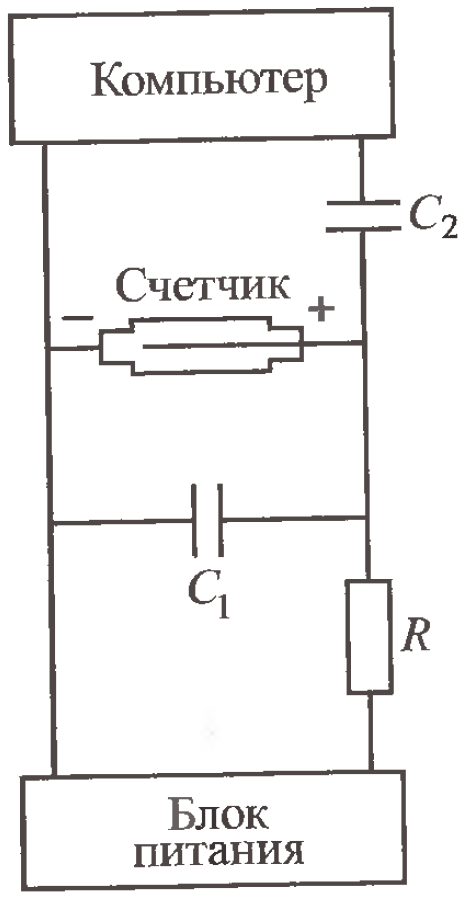
\includegraphics[width=.2\textwidth]{shema.png}
\caption{Схема включения счетчика}
\end{wrapfigure}

В любой физической лаборатории всегда присутствует радиоактивное излучение. Это излучение является радиоактивным фоном, с которым складывается излучение других источников, если они присутствуют. Основную часть фона обычно составляет космическое излучение.\par
Устройство счетчика Гейгера-Мюллера: наполненный газом металлический цилиндр с двумя электродами. Катод - корпус счетчика. Анод - тонкая нить, натянутая вдоль оси цилиндрического корпуса. Необходимое напряжение (400 В) подаётся на счётчик от смонтированного вместе с ним блока питания через повышающий трансформатор. (рис.1)

Космические частицы — в основном, протоны (92\%), альфа-частицы
(6\%) и электроны/позитроны (1\%) — ионизуют газ, которым наполнен счётчик, а также выбивают электроны из его стенок. Двигаясь в сильном электрическом ноле между электродами счётчика, образовавшиеся электроны соударяются с молекулами газа, выбивая из них новые. В результате образуется целая лавина электронов, через счётчик протекает кратковременный импульс тока (разряд). Этот импульс и регистрируется установкой, оцифровывается платой аналоговоцифрового преобразователя, и информация о нём через USB интерфейс подаётся на компьютер.\par

Число зарегистрированных частиц зависит от времени измерения, размеров счётчика, от давления и состава газа и от материала, из которого сделаны стенки счётчика.

\subsection{Базовые погрешности}
Наиболее важной характеристикой является среднее число регистрируемых частиц в единицу времени. Если $n_{1}, n_{2}, ..., n_{N}$ - результаты N проведённых в одинаковых условиях измерений, можно вычислить выборочное среднее значение числа измерений:
\[\langle n \rangle = \frac{1}{N}\sum\limits_{i=1}^{N} n_{i}\]
Если продолжать проводить измерения, можно ожидать, что выборочное среднее будет стремиться к некоторому конечному пределу, который можно назвать «истинным» средним значением числа регистрируемых частиц(т.к. в реальном эксперименте N конечно, то возникает погрешность):
\[\overline{n} = \lim_{N \to \infty} \langle n \rangle\]
Количественно меру флуктуаций среднего значения от опыта к опыту принято измерять среднеквадратичным (или стандартным) отклонением $\sigma_{n}$
По определению, средний квадрат отклонения, называемый также дисперсией, равен:
\[\sigma_{n}^2 = \frac{1}{N}\sum\limits_{i=1}^{N} (n_{i} - \langle n \rangle)^2 = \langle (n_{i} - \langle n \rangle)^2 \rangle\]
Погрешность среднего значения $\langle n \rangle$ при независимых измерениях связана с погрешностью отдельного измерения формулой:
\[\sigma_{\langle n \rangle} = \frac{\sigma_{n}}{\sqrt{N}}\]
Таким образом, увеличивая количество измерений, среднее значение приближается к «истинному» n. При конечном N истинное среднее с высокой вероятностью лежит в интервале 
\[\overline{n} = \langle n \rangle \pm \frac{\sigma_{n}}{\sqrt{N}}\]

\subsection{Пуассоновский процесс}
Если события однородны во времени и каждое следующее событие не зависит от прошлого, то последовательность таких событий называют \textit{пуассоновский процессом}.\newline

\begin{figure}[t]
    \centering
    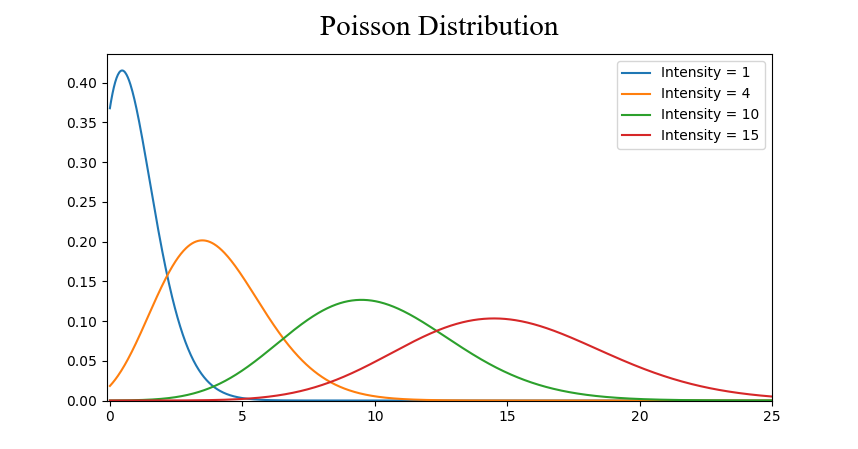
\includegraphics[width=0.6\textwidth]{process.png}
    \caption{График распределения Пуассона}
\end{figure}

Вероятности $\omega_{n}$ того, что в эксперименте будет обнаружено n частиц, для распределения Пуассона имеют вид:
\[\omega_{n} =  \frac{\overline{n}^{n}}{n!} e^{-\overline{n}}\]
\newline
При больших $\overline{n} > 10$ график распределения (рис.2) стремиться к гладкой симметричной кривой, быстро убывающей к нулю при отдалении от центра.
\newline
Для пуассоновского процесса справедливо равенство:
\[\sigma = \sqrt{\overline{n}}\]
То есть среднеквадратичное отклонение равно корню из среднего. На практике можно ожидать приближённое равенство для выборочных значений:
\[\sigma_{n} \approx \sqrt{\langle n \rangle}\]
При больших $\overline{n}$ распределение Пуассона переходит в так называемое нормальное распределение или распределение Гаусса, которое выражается через $\overline{n}, n$ и среднеквадратическое отклонение $\sigma_{n}$:
\[\rho_{n} = \frac{1}{\sqrt{2\pi}\sigma_{n}}e^{-\frac{(n - \overline{n})^2}{2\sigma_{n}^2}}\]
\section{Погрешность эксперимента}

Если подставить основное свойство распределения Пуассона в формулу погрешности среднего значения, то получится среднеквадратичная погрешность определения среднего:
\[\sigma_{\langle n \rangle} = \frac{\sigma_{n}}{\sqrt{N}} = \sqrt{\frac{\langle n \rangle}{N}}\]
Для относительного значения погрешности:
\[\varepsilon_{\langle n \rangle} = \frac{\sigma_{\langle n \rangle}}{\langle n \rangle} = \frac{1}{\sqrt{\langle n \rangle N}}\]

Рассмотрим опыт, в котором интервал измерения t разбит на $N = \frac{t}{\tau}$ промежутков, длительностью $\tau$. В знаменателе полученного выражения, как нетрудно видеть, стоит полное число частиц $N_{0} = \langle n \rangle N = \sum\limits_{i=1}^{N} n_{i}$, зарегистрированных за всё время измерений t. То есть относительная погрешность опыта не зависит от интервалов $\tau$ разбиения серий, и убывает обратно пропорционально корню из общего числа частиц $N_{0}$.

Таким образом, единственный способ увеличить точность опыта — увеличивать общее число регистрируемых частиц за счёт увеличения совокупного времени измерений $\tau$.

\section{Обработка результатов}
\subsection{Вычисление погрешностей}

В данном эксперименте будут обработанны данные для 3х времен: $\tau = 10\text{с}, \tau = 20\text{с}, \tau = 40\text{с}$. В силу ограниченности цифровой обработкой, распределения Пуассона и Гаусса будут построенны только для $\tau = 20\text{с}, \tau = 40\text{с}$

Далее в таблицах 1,2 приведенны данные полученные прибором для $\tau = 20\text{с}, \tau = 40\text{с}$, в таблицах 3,4,5 данные для гистограммы полученные на основе данных из таблиц 1,2 для $\tau = 10\text{с}, \tau = 20\text{с}, \tau = 40\text{с}$. В таблицах 6,7 содержатся данные для гистограммы об распределении Пуассона и Гаусса полученных на основе таблиц 1-5 при  $\tau = 20\text{с}, \tau = 40\text{с}$. Таблица 8 содержит сравнение отклонений долей случаев от средних значений с теоретическими оценками. 

Рисунки 3-5 содержат гистограммы зависимости долей случаев от числа случаев. Рисунки 3,4 содержат также распределения Пуассона и Гаусса для данных параметров, для оценки погрешности.

Вычислим среднее число срабатываний счетчика за 10с,20с,40с:
\[\overline{n_{10}} = \frac{1}{10}\sum\limits_{i=1}^{10} n_{i} \approx 13,22\]
\[\overline{n_{20}} = \frac{1}{20}\sum\limits_{i=1}^{20} n_{i} \approx 26,48\]
\[\overline{n_{40}} = \frac{1}{40}\sum\limits_{i=1}^{40} n_{i} \approx 52,96\]
Вычислим среднеквадратическую погрешность отдельного измерения для 10с,20с,40с:
\[\sigma_{n_{10}} = \sqrt{\frac{1}{10}\sum\limits_{i=1}^{10} (n_{i} - \overline{n_{10}})^2} \approx 3,53\]
\[\sigma_{n_{20}} = \sqrt{\frac{1}{20}\sum\limits_{i=1}^{20} (n_{i} - \overline{n_{20}})^2} \approx 4,76\]
\[\sigma_{n_{40}} = \sqrt{\frac{1}{40}\sum\limits_{i=1}^{40} (n_{i} - \overline{n_{40}})^2} \approx 6,06\]
Рассчитаем среднеквадратическое отклонение по свойству процесса Пуассона и сравним с стандартной:
\[\sigma_{n_{10}} = \sqrt{\overline{n_{10}}} \approx 3,64 \pm 3,53\]
\[\sigma_{n_{20}} = \sqrt{\overline{n_{20}}} \approx 5,15 \pm 4,76\]
\[\sigma_{n_{40}} = \sqrt{\overline{n_{40}}} \approx 7,28 \pm 6,06\]
Определим долю случаев, когда отклонения от среднего значения не превышают $\sigma_{n}$ и $2\sigma_{n}$ и сравним с теоретическими оценками - Таблица 8.
Рассчитаем погрешность среднего значения $\sigma_{\langle n \rangle} = \frac{\sigma_{n}}{\sqrt{N}}$:
\[\sigma_{\langle n_{10} \rangle} = \frac{\sigma_{n_{10}}}{\sqrt{10}} \approx 0,18\]
\[\sigma_{\langle n_{20} \rangle} = \frac{\sigma_{n_{20}}}{\sqrt{20}} \approx 0,33\]
\[\sigma_{\langle n_{20} \rangle} = \frac{\sigma_{n_{20}}}{\sqrt{20}} \approx 0,606\]
Для каждого $\tau$ вычислим среднюю интенсивность регистрируемых частиц в секунду $\overline{j} = \frac{\overline{n}}{\tau}$ и её погрешность 
$\sigma_{j} = \frac{\sigma_{n}}{\tau}$:
\[\langle j_{10} \rangle = \frac{\overline{n_{10}}}{10} \approx 1,32\]
\[\sigma_{j_{10}} = \frac{\sigma_{\langle n_{10} \rangle}}{10} \approx 0,018\]
\[\overline{j_{10}} = \langle j_{10} \rangle \pm \sigma_{j_{10}} = 1,32 \pm 0,018 \]
\[\langle j_{20} \rangle = \frac{\overline{n_{20}}}{20} \approx 1,32\]
\[\sigma_{j_{20}} = \frac{\sigma_{\langle n_{20} \rangle}}{20} \approx 0,017\]
\[\overline{j_{20}} = \langle j_{20} \rangle \pm \sigma_{j_{20}} = 1,32 \pm 0,018 \]
\[\langle j_{40} \rangle = \frac{\overline{n_{40}}}{40} \approx 1,32\]
\[\sigma_{j_{40}} = \frac{\sigma_{\langle n_{40} \rangle}}{40} \approx 0,015\]
\[\overline{j_{40}} = \langle j_{40} \rangle \pm \sigma_{j_{40}} = 1,32 \pm 0,018 \]
Заметим, что средняя интенсивность регистрируемых частиц в секунду не зависит от величины интервала $\tau$ и числа точек N.

Обработаем данные из вышевычисленных и таблиц с данными и построим гистограммы зависимости долей случаев от их числа. Экспериментальные гистограммы (рисунки 3-5) с большой точностью согласуются с распределениями Пуассона и с несколько меньшей точностью с распределением Гаусса. 

Из таблицы 8 и сравнения гистограмм 4,5 можно сделать вывод, что при достаточно больших N распределение Пуассона приближается к нормальному распределению (распределению Гаусса).

\subsection{Вывод}
В ходе выполнения работы познакомился с основными понятиями статистики. Определил среднее число регистрируемых космических лучей в секунду и определил погрешность результата. Выяснил, что средняя интенсивность регистрируемых частиц в секунду не зависит от величины интервала $\tau$ и числа точек N. Исследовал Пуассоновский процесс и распределение Гаусса.\par



\newpage



\section{Данные, таблицы и гистограммы}
\begin{table}[!h]
\begin{center}
\begin{tabular}{|l|l|l|l|l|l|l|l|l|l|l|}
\hline
        & 0  & 1  & 2  & 3  & 4  & 5  & 6  & 7  & 8  & 9  \\ \hline
0       & 33 & 18 & 36 & 25 & 31 & 23 & 25 & 26 & 24 & 20 \\ \hline
10      & 19 & 29 & 36 & 21 & 23 & 18 & 27 & 28 & 37 & 24 \\ \hline
20      & 32 & 35 & 17 & 30 & 24 & 22 & 22 & 27 & 29 & 25 \\ \hline
30      & 22 & 22 & 17 & 29 & 27 & 30 & 28 & 31 & 26 & 19 \\ \hline
40      & 30 & 29 & 27 & 22 & 24 & 28 & 21 & 39 & 29 & 33 \\ \hline
50      & 35 & 21 & 24 & 24 & 26 & 23 & 24 & 22 & 28 & 18 \\ \hline
60      & 24 & 27 & 36 & 24 & 29 & 28 & 22 & 40 & 26 & 16 \\ \hline
70      & 30 & 24 & 21 & 32 & 26 & 20 & 26 & 31 & 31 & 28 \\ \hline
80      & 24 & 29 & 25 & 25 & 26 & 20 & 32 & 21 & 22 & 38 \\ \hline
90      & 29 & 26 & 28 & 22 & 30 & 24 & 27 & 31 & 32 & 36 \\ \hline
100     & 25 & 25 & 29 & 27 & 23 & 30 & 28 & 28 & 16 & 28 \\ \hline
110     & 27 & 24 & 26 & 26 & 27 & 33 & 23 & 21 & 23 & 25 \\ \hline
120     & 28 & 31 & 37 & 27 & 34 & 24 & 28 & 33 & 30 & 23 \\ \hline
130     & 29 & 30 & 27 & 23 & 27 & 24 & 23 & 23 & 31 & 32 \\ \hline
140     & 27 & 20 & 23 & 28 & 25 & 24 & 23 & 26 & 23 & 23 \\ \hline
150     & 23 & 26 & 28 & 27 & 29 & 22 & 25 & 34 & 24 & 30 \\ \hline
160     & 28 & 21 & 33 & 23 & 22 & 28 & 31 & 22 & 34 & 29 \\ \hline
170     & 25 & 32 & 16 & 31 & 19 & 32 & 32 & 24 & 30 & 19 \\ \hline
180     & 33 & 24 & 27 & 27 & 22 & 22 & 33 & 29 & 18 & 21 \\ \hline
190     & 25 & 31 & 30 & 24 & 19 & 24 & 29 & 30 & 31 & 26 \\ \hline
\end{tabular}
\caption{Число срабатываний счетчика за $\tau = 20$ с}
\end{center}
\end{table}

\begin{table}[!h]
\begin{center}
\begin{tabular}{|l|l|l|l|l|l|l|l|l|l|l|}
\hline
   & 1  & 2  & 3  & 4  & 5  & 6  & 7  & 8  & 9  & 10 \\ \hline
0  & 51 & 61 & 54 & 51 & 44 & 48 & 57 & 41 & 55 & 61 \\ \hline
10 & 67 & 47 & 46 & 49 & 54 & 44 & 46 & 57 & 59 & 45 \\ \hline
20 & 59 & 49 & 52 & 60 & 62 & 56 & 48 & 49 & 46 & 46 \\ \hline
30 & 51 & 60 & 57 & 62 & 42 & 54 & 53 & 46 & 57 & 59 \\ \hline
40 & 53 & 50 & 46 & 53 & 60 & 55 & 50 & 54 & 58 & 68 \\ \hline
50 & 50 & 56 & 53 & 56 & 44 & 51 & 52 & 60 & 44 & 48 \\ \hline
60 & 59 & 64 & 58 & 61 & 53 & 59 & 50 & 51 & 46 & 63 \\ \hline
70 & 47 & 51 & 49 & 49 & 46 & 49 & 55 & 51 & 59 & 54 \\ \hline
80 & 49 & 56 & 50 & 53 & 63 & 57 & 47 & 51 & 56 & 49 \\ \hline
90 & 57 & 54 & 44 & 62 & 39 & 56 & 54 & 43 & 59 & 57 \\ \hline
\end{tabular}
\caption{Число срабатываний счетчика за $\tau = 40$ с}
\end{center}
\end{table}

\begin{table}[!h]
\begin{center}
\begin{tabular}{|l|l|}
\hline
Число импульсов, $n_{i}$ & Доля случаев, $\omega_{n}$ \\ \hline
4                        & 0.0025                     \\ \hline
5                        & 0.0025                     \\ \hline
6                        & 0.0175                     \\ \hline
7                        & 0.0225                     \\ \hline
8                        & 0.045                      \\ \hline
9                        & 0.0475                     \\ \hline
10                       & 0.0725                     \\ \hline
11                       & 0.095                      \\ \hline
12                       & 0.105                      \\ \hline
13                       & 0.16                       \\ \hline
14                       & 0.1125                     \\ \hline
15                       & 0.0975                     \\ \hline
16                       & 0.0625                     \\ \hline
17                       & 0.04                       \\ \hline
18                       & 0.0375                     \\ \hline
19                       & 0.0325                     \\ \hline
20                       & 0.01                       \\ \hline
21                       & 0.02                       \\ \hline
22                       & 0.005                      \\ \hline
23                       & 0.005                      \\ \hline
24                       & 0.005                      \\ \hline
25                       & 0.0025                     \\ \hline
\end{tabular}
\caption{Данные для гистограммы распределение при $\tau = 10$ с}
\end{center}
\end{table}

\begin{table}[!h]
\begin{center}
\begin{tabular}{|l|l|}
\hline
Число импульсов, $n_{i}$ & Доля случаев, $\omega_{n}$ \\ \hline
16                       & 0.015                      \\ \hline
17                       & 0.01                       \\ \hline
18                       & 0.02                       \\ \hline
19                       & 0.025                      \\ \hline
20                       & 0.02                       \\ \hline
21                       & 0.04                       \\ \hline
22                       & 0.07                       \\ \hline
23                       & 0.08                       \\ \hline
24                       & 0.105                      \\ \hline
25                       & 0.06                       \\ \hline
26                       & 0.065                      \\ \hline
27                       & 0.08                       \\ \hline
28                       & 0.08                       \\ \hline
29                       & 0.07                       \\ \hline
30                       & 0.06                       \\ \hline
31                       & 0.055                      \\ \hline
32                       & 0.04                       \\ \hline
33                       & 0.035                      \\ \hline
34                       & 0.015                      \\ \hline
35                       & 0.01                       \\ \hline
36                       & 0.02                       \\ \hline
37                       & 0.01                       \\ \hline
38                       & 0.005                      \\ \hline
39                       & 0.005                      \\ \hline
40                       & 0.005                      \\ \hline
\end{tabular}
\caption{Данные для гистограммы распределение при $\tau = 20$ с}
\end{center}
\end{table}

\begin{table}[!h]
\begin{center}
\begin{tabular}{|l|l|}
\hline
Число импульсов, $n_{i}$ & Доля случаев, $\omega_{n}$ \\\hline
41                       & 0.01                       \\\hline
42                       & 0.01                       \\\hline
43                       & 0.01                       \\\hline
44                       & 0.05                       \\\hline
45                       & 0.01                       \\\hline
46                       & 0.08                       \\\hline
47                       & 0.03                       \\\hline
48                       & 0.03                       \\\hline
49                       & 0.08                       \\\hline
50                       & 0.05                       \\\hline
51                       & 0.08                       \\\hline
52                       & 0.02                       \\\hline
53                       & 0.06                       \\\hline
54                       & 0.07                       \\\hline
55                       & 0.03                       \\\hline
56                       & 0.06                       \\\hline
57                       & 0.07                       \\\hline
58                       & 0.02                       \\\hline
59                       & 0.07                       \\\hline
60                       & 0.04                       \\\hline
61                       & 0.03                       \\\hline
62                       & 0.03                       \\\hline
63                       & 0.02                       \\\hline
64                       & 0.01                       \\\hline
65                       & 0.0                        \\\hline
66                       & 0.0                        \\\hline
67                       & 0.01                       \\\hline
68                       & 0.01                      \\\hline
\end{tabular}
\caption{Данные для гистограммы распределение при $\tau = 40$ с}
\end{center}
\end{table}

\begin{table}[!h]
\begin{center}
\begin{tabular}{|l|l|l|}
\hline
Число импульсов, $n_{i}$ & Доля случаев при распределении Пуассона, $\omega_{n}$ & Доля случаев при распределении Гаусса, $\rho_{n}$ \\ \hline
16                       & 0.008829787                                           & 0.010199903                                       \\ \hline
17                       & 0.013753691                                           & 0.014707503                                       \\ \hline
18                       & 0.020233208                                           & 0.020443521                                       \\ \hline
19                       & 0.028198703                                           & 0.027393423                                       \\ \hline
20                       & 0.037335083                                           & 0.035384314                                       \\ \hline
21                       & 0.047077761                                           & 0.044060468                                       \\ \hline
22                       & 0.056664506                                           & 0.052888505                                       \\ \hline
23                       & 0.065238092                                           & 0.061199424                                       \\ \hline
24                       & 0.071979361                                           & 0.068266437                                       \\ \hline
25                       & 0.076240539                                           & 0.073407596                                       \\ \hline
26                       & 0.077648057                                           & 0.076093686                                       \\ \hline
27                       & 0.076152613                                           & 0.076037897                                       \\ \hline
28                       & 0.072018614                                           & 0.073246256                                       \\ \hline
29                       & 0.065760445                                           & 0.068016554                                       \\ \hline
30                       & 0.058044552                                           & 0.060886033                                       \\ \hline
31                       & 0.049581282                                           & 0.052540547                                       \\ \hline
32                       & 0.041028511                                           & 0.043706432                                       \\ \hline
33                       & 0.032922272                                           & 0.035048544                                       \\ \hline
34                       & 0.02564064                                            & 0.027093709                                       \\ \hline
35                       & 0.019398976                                           & 0.020190209                                       \\ \hline
36                       & 0.014269024                                           & 0.014503974                                       \\ \hline
37                       & 0.010211994                                           & 0.010044009                                       \\ \hline
38                       & 0.007116147                                           & 0.006705034                                       \\ \hline
39                       & 0.004831681                                           & 0.00431488                                        \\ \hline
40                       & 0.003198573                                           & 0.002676766                                       \\ \hline
\end{tabular}
\caption{Данные для гистограммы распределение Пуассона и Гаусса при $\tau = 20$ с}
\end{center}
\end{table}

\begin{table}[!h]
\begin{center}
\begin{tabular}{|l|l|l|}
\hline
Число импульсов, $n_{i}$ & Доля случаев при распределении Пуассона, $\omega_{n}$ & Доля случаев при распределении Гаусса, $\rho_{n}$ \\ \hline
41                       & 0.014361584                                           & 0.003572789                                       \\ \hline
42                       & 0.018109274                                           & 0.005923482                                       \\ \hline
43                       & 0.022303887                                           & 0.009396956                                       \\ \hline
44                       & 0.026845769                                           & 0.014263879                                       \\ \hline
45                       & 0.031594488                                           & 0.020717075                                       \\ \hline
46                       & 0.036374871                                           & 0.028791185                                       \\ \hline
47                       & 0.040987514                                           & 0.038285206                                       \\ \hline
48                       & 0.045222891                                           & 0.048712764                                       \\ \hline
49                       & 0.048877639                                           & 0.059305488                                       \\ \hline
50                       & 0.051771195                                           & 0.069085567                                       \\ \hline
51                       & 0.053760833                                           & 0.07700521                                        \\ \hline
52                       & 0.054753341                                           & 0.082128374                                       \\ \hline
53                       & 0.054712017                                           & 0.08381209                                        \\ \hline
54                       & 0.053658304                                           & 0.081839025                                       \\ \hline
55                       & 0.051668069                                           & 0.076463568                                       \\ \hline
56                       & 0.048863231                                           & 0.068357947                                       \\ \hline
57                       & 0.045399942                                           & 0.058474133                                       \\ \hline
58                       & 0.041454844                                           & 0.047860684                                       \\ \hline
59                       & 0.037210992                                           & 0.037483001                                       \\ \hline
60                       & 0.032844902                                           & 0.028088602                                       \\ \hline
61                       & 0.028515837                                           & 0.020140314                                       \\ \hline
62                       & 0.024358044                                           & 0.013817921                                       \\ \hline
63                       & 0.020476222                                           & 0.00907109                                        \\ \hline
64                       & 0.016944074                                           & 0.005697923                                       \\ \hline
65                       & 0.01380551                                            & 0.003424633                                       \\ \hline
66                       & 0.011077876                                           & 0.001969481                                       \\ \hline
67                       & 0.008756482                                           & 0.001083752                                       \\ \hline
68                       & 0.006819754                                           & 0.000570622                                       \\ \hline
\end{tabular}
\caption{Данные для гистограммы распределение Пуассона и Гаусса при $\tau = 40$ с}
\end{center}
\end{table}

\begin{table}[!h]
\begin{center}
\begin{tabular}{|l|l|l|l|}
\hline
Ошибка                             & Число случаев & Доля случаев, \% & Теоретическая оценка \\ \hline
$\pm\sigma_{n_{20}} = \pm 4,76$    & 145           & 72,5             & 68                   \\ \hline
$\pm 2\sigma_{n_{20}} = \pm 9,52$  & 188           & 94               & 95                   \\ \hline
$\pm 3\sigma_{n_{20}} = \pm 14,28$ & 200           & 100              & 99                   \\ \hline
$\pm\sigma_{n_{40}} = \pm 6,06$    & 67            & 67               & 68                   \\ \hline
$\pm 2\sigma_{n_{40}} = \pm 12,12$ & 97            & 97               & 95                   \\ \hline
$\pm 3\sigma_{n_{40}} = \pm 18,18$ & 100           & 100              & 99                   \\ \hline
\end{tabular}
\caption{Оценка распределения доли случаев}
\end{center}
\end{table}

\begin{figure}[t]
    \centering
    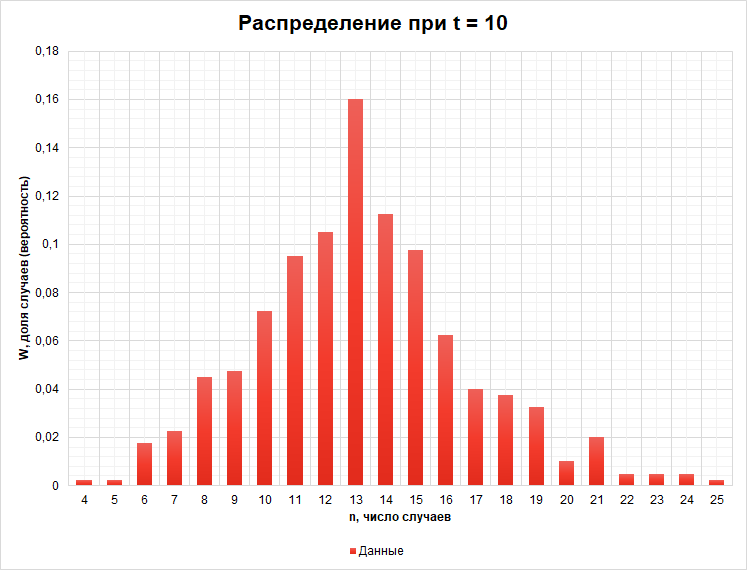
\includegraphics[width=1\textwidth]{t10}
    \caption{Гистограмма с данными при $\tau = 10$}
\end{figure}

\begin{figure}[t]
    \centering
    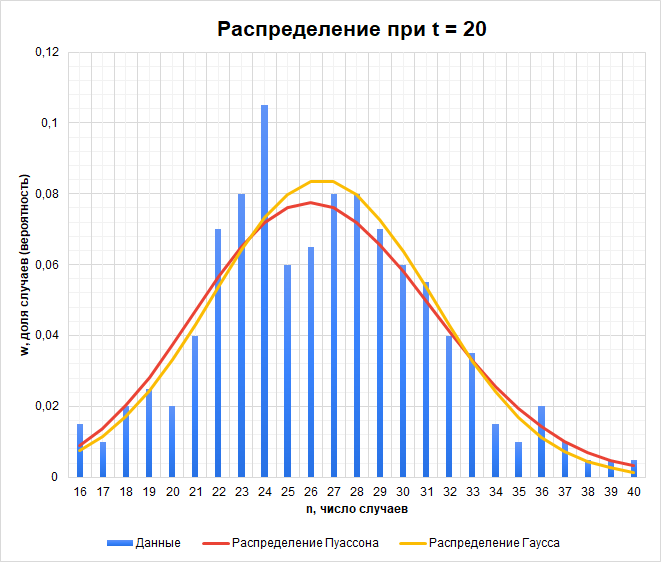
\includegraphics[width=1\textwidth]{t20}
    \caption{Гистограмма с данными и распределениями Пуассона и Гаусса при $\tau = 20$}
\end{figure}

\begin{figure}[t]
    \centering
    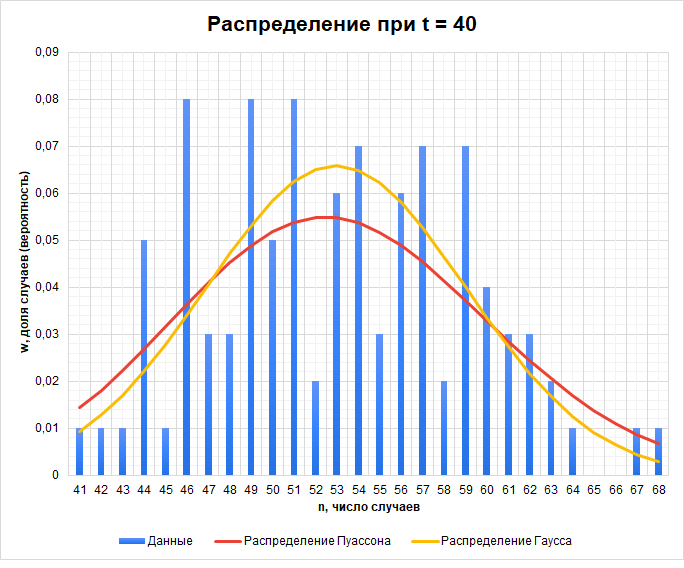
\includegraphics[width=1\textwidth]{t40}
    \caption{Гистограмма с данными и распределениями Пуассона и Гаусса при $\tau = 40$}
\end{figure}

\end{document}